\documentclass[a4paper]{article}

\usepackage[english]{babel}
\usepackage[utf8]{inputenc}
\usepackage{amsmath}
\usepackage{graphicx}
\usepackage[colorinlistoftodos]{todonotes}

\title{Your Paper}

\author{You}

\date{\today}

\begin{document}
\maketitle

\begin{abstract}
Your abstract.
\end{abstract}

\section{Introduction}

Your introduction goes here! Some examples of commonly used commands and features are listed below, to help you get started. If you have a question, please use the help menu (``?'') on the top bar to search for help or ask us a question.

\section{Some \LaTeX{} Examples}
\label{sec:examples}

\subsection{How to Leave Comments}

Comments can be added to the margins of the document using the \todo{Here's a comment in the margin!} todo command, as shown in the example on the right. You can also add inline comments:

\todo[inline, color=green!40]{This is an inline comment.}

\subsection{How to Include Figures}

First you have to upload the image file (JPEG, PNG or PDF) from your computer to writeLaTeX using the upload link the project menu. Then use the includegraphics command to include it in your document. Use the figure environment and the caption command to add a number and a caption to your figure. See the code for Figure \ref{fig:frog} in this section for an example.

\begin{figure}
\centering
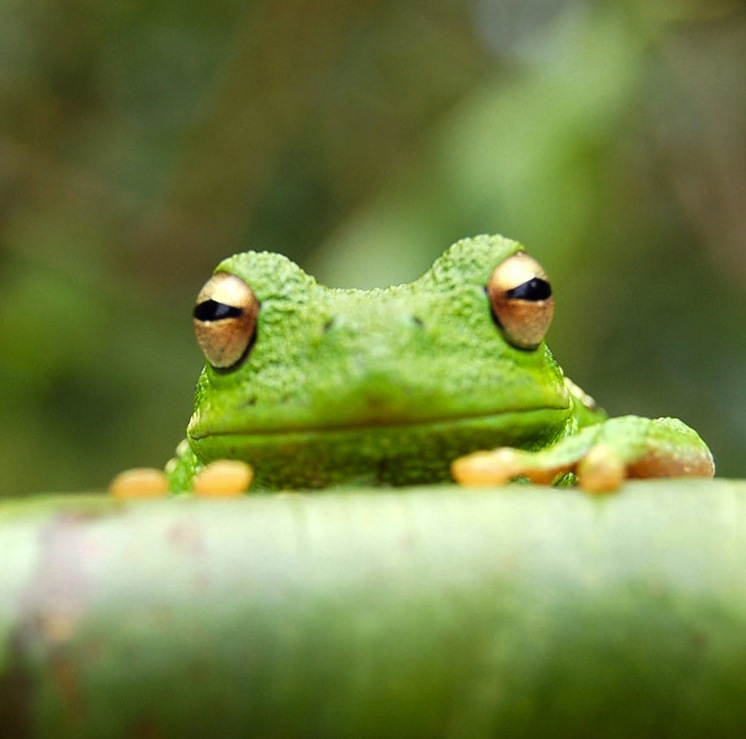
\includegraphics[width=0.3\textwidth]{frog.jpg}
\caption{\label{fig:frog}This frog was uploaded to writeLaTeX via the project menu.}
\end{figure}

\subsection{How to Make Tables}

Use the table and tabular commands for basic tables --- see Table~\ref{tab:widgets}, for example.

\begin{table}
\centering
\begin{tabular}{l|r}
Item & Quantity \\\hline
Widgets & 42 \\
Gadgets & 13
\end{tabular}
\caption{\label{tab:widgets}An example table.}
\end{table}

\subsection{How to Write Mathematics}

\LaTeX{} is great at typesetting mathematics. Let $X_1, X_2, \ldots, X_n$ be a sequence of independent and identically distributed random variables with $\text{E}[X_i] = \mu$ and $\text{Var}[X_i] = \sigma^2 < \infty$, and let
$$S_n = \frac{X_1 + X_2 + \cdots + X_n}{n}
      = \frac{1}{n}\sum_{i}^{n} X_i$$
denote their mean. Then as $n$ approaches infinity, the random variables $\sqrt{n}(S_n - \mu)$ converge in distribution to a normal $\mathcal{N}(0, \sigma^2)$.

\subsection{How to Make Sections and Subsections}

Use section and subsection commands to organize your document. \LaTeX{} handles all the formatting and numbering automatically. Use ref and label commands for cross-references.

\subsection{How to Make Lists}

You can make lists with automatic numbering \dots

\begin{enumerate}
\item Like this,
\item and like this.
\end{enumerate}
\dots or bullet points \dots
\begin{itemize}
\item Like this,
\item and like this.
\end{itemize}
\dots or with words and descriptions \dots
\begin{description}
\item[Word] Definition
\item[Concept] Explanation
\item[Idea] Text
\end{description}

We hope you find write\LaTeX\ useful, and please let us know if you have any feedback using the help menu above.

\end{document}